\clearpage
\section{Other Requirements} 
\hspace{0.5cm} 

\subsection{Quiz Print View}
\subsubsection{Problem Statement}
	Generate a printable view of quiz with or without answers

\subsubsection{Why Do we need this?}
	Many times its necessary to discuss the questions with the students after the quiz along with the correct answers. There wasn't a simple view which showed all the questions along with their answers in a simple format. Also for some quizzes there were students who wanted to take the quiz offline. A printable page with just the questions would allow the instructor to conduct the quiz using the app and offline simultaneously.

\subsubsection{Implementation}
	Displaying of question has two parts - the question text and the answers. Getting the Question text is straight forward and is directly obtained from the database field. Answers depends on the type of question

    \begin{itemize}
        \item Integer question - Directly print the answer
	    \item Single and multiple answer question - Print the options and put a tick symbol on the answer
	    \item Fill in the blanks question - List all possible answers separated by comma
	    \item Floating point type question - Print the possible range of answers in the form of <lower bound> to <upper bound>
	\end{itemize}

\begin{figure}[h!]
\begin{center}
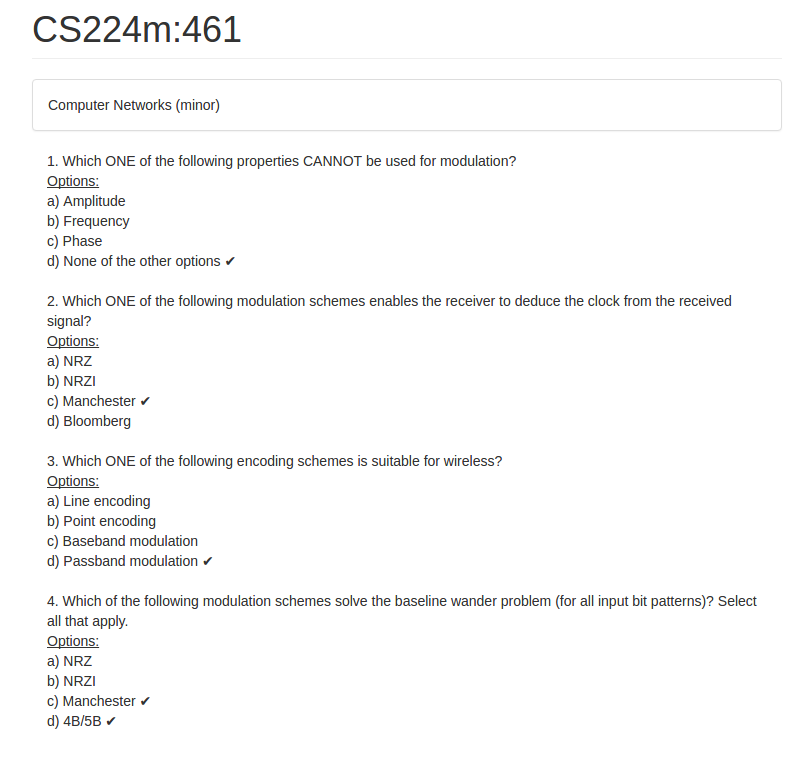
\includegraphics[scale=.4]{diagrams/print-view} 
\vspace{1cm}
\caption{Print View of Quiz}
\end{center}
\end{figure}

\subsection{Instructor Profile Page}
\subsubsection{Problem Statement}
	Create a My Account page for instructor which allows them to change their personal details and passowrd

\subsubsection{Implementation}
	Saving of personal details is a direct update to the database entry. Password is hashed using BCRYPT hashing method and then saved to the database. 

\subsection{Reason texts list page}
\subsubsection{Problem Statement}
	Create a page to list all reason texts given by students grouped by the question

\subsubsection{Why do we need this?}
	Reason text is a feature using which students can explain the reason behind their answer, or how they arrived at their answers. This is userful in many cases where the students needs to be evaluated for his methodoloty of solving the problem or reasoning. Displaying a list of all the reasons texts given by the students along with the Quiz Statistics feature 4allows to instructor to know how and why the students chose a particular answer.

\subsubsection{Implementation}
	We iterate over the submissions for the particular quiz and create a dictionary with the key as the question_id and the value as a list of reasons given for the particular question	

\begin{figure}[h!]
\begin{center}
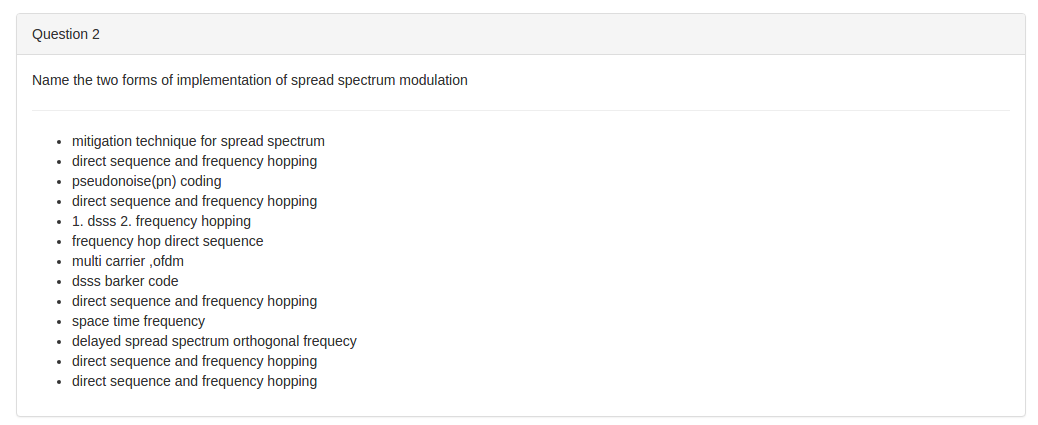
\includegraphics[scale=.4]{diagrams/reasons-list} 
\vspace{1cm}
\caption{Reasons list page}
\end{center}
\end{figure}